%!TEX root = ../../thesis.tex

\section{Derivation of the $\tau$-decay ratio}
One of the central formulas of our QCD $\tau$-decay analysis is the $\tau$-decay ratio
\begin{equation}
	R_\tau = 12 \pi S_{EW} \int_0^{m_\tau^2} \frac{\diff s}{m_\tau^2} \left(1 - \frac{s}{m_\tau^2} \right)^2 \left[ \left( 1 + 2 \frac{s}{m_\tau^2} \right) \Im \Pi^{(1)} (s) + \Im \Pi^{(0)} (s) \right].
\end{equation}
It was originally derived by Tsai in 1971 \cite{Tsai1971} and will be probed in the following the guide of \cite{Schwab2002}.

First we need to remember the Lorentz-decomposition of the QCD correlator
\begin{equation}
	\label{eq:appTauLorentzDecomposition}
	\Pi_{\mu\nu} (q) = (q_\mu q_\nu - q^2 g_{\mu\nu}) \Pi^{(T)}(q^2) + q^\mu q^\nu \Pi^{(L)} (q^2).
\end{equation}
The desired decay-ratio can be expressed as
\begin{equation}
	R_\tau = \frac{\Gamma(\tau \to hadrons)}{\Gamma(\tau\to e \nu_\tau \bar \nu_e)}
\end{equation}
so we need to make use of the general decay-rate defined as
\begin{equation}
	\Gamma = \frac{1}{2 M_A} \int \left( \Pi_f \frac{\diff^3 p}{(2\pi)^3} \frac{1}{2 E_f} \right) | \mathcal{M} (A \to \sum_f f) |^2 (2\pi)^4 \delta(p_A - \sum_f p_f),
\end{equation}
where $|\mathcal{M}|^2$ is the squared decay matrix element.
As we do not know all the corrections of quark interactions within the $\tau$-decay we want to make use of the optical theorem. The optical theorem states that the before mentioned squared decay matrix element $|\mathcal{M}|^2$, as in Fig. \ref{fig:tauOpticalTheorem} b), is twice the imaginary part of two times the diagram, like in Fig. \ref{fig:tauOpticalTheorem} a). Consequently we will calculate the squared decay matrix element of a) in \ref{fig:tauOpticalTheorem} and use its imaginary part, dividing by a factor of two to get to the needed $\tau$ decay rate. Within the $\tau$-decay rate we furthermore have to sum over all possible hadronic final states and integrate over their phase space factors to deal with the momentum-$\delta$, leaving us with an integration over the $\tau$-neutrino.
\begin{figure}[t]
	\label{fig:tauOpticalTheorem}
	\centering
	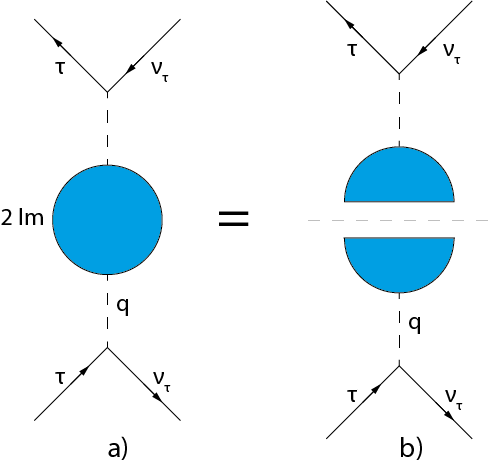
\includegraphics[width=0.6\textwidth]{img/appendix/tauOpticalTheorem.png}
	\caption{The optical theorem relates the imaginary part of a) to the the hadronic $\tau$ decay b). The blue areas, indicate higher order interactions.}
\end{figure}

Starting with the diagrammatical evaluation of Fig. \ref{fig:tauOpticalTheorem} a), making use of of the Feynman rules, we get
\begin{equation}
	\label{eq:tauOpticalAmplitude}
	\begin{split}
		i \mathcal{M} &= (-i)^2 \frac{g^2}{2} \bar u(p_\tau) \gamma_\nu \left(\frac{1-\gamma^5}{2}\right) u(p_{\nu_\tau}) \frac{-i}{M_W^2} \left(\frac{i}{4}\frac{g^2}{2} \Pi^{\mu\nu}(q)\right) \\
		&\times \frac{-i}{M_W^2} \bar(p_{\nu_\tau}) \gamma_\nu \left( \frac{1-\gamma^5}{2} \right) u(p_\tau).
	\end{split}
\end{equation}
Focusing on the spinors, while summing over the spins we can evaluate the traces
\begin{align}
		&\frac{1}{2} \sum_{spins} \bar u (p_\tau) \gamma_\mu \left(\frac{1-\gamma^5}{2}\right) u(p_{\nu_\tau}) \bar u(p_{\nu_\tau}) \gamma_\nu \left(\frac{1-\gamma^5}{2}\right) u(p_\tau) \\
		=\quad& \frac{1}{2} \Tr \left[ \slashed p_\tau \gamma_\mu \left(\frac{1-\gamma^5}{2} \right) \slashed p_{\nu_\tau} \gamma_\nu \left(\frac{1-\gamma^5}{2} \right) \right]\\
		=\quad&\frac{1}{2} \Tr \left[ \slashed p_\tau \gamma_\mu \slashed p_{\nu_\tau} \gamma_\nu \left( \frac{1 - \gamma^5}{2} \right) \right] \\
		=\quad & (p^\mu_\tau p_{\nu_\tau}^\nu + p_\tau^\nu p_{\nu_\tau}^\mu - g^{\mu\nu} p_{\nu_\tau} \dot p_\tau - i \epsilon^{\alpha\mu\beta\nu}p_{\tau, \alpha} p_{{\nu_\tau}, \beta} ),
\end{align}
which then have to be dotted into \eqref{eq:tauOpticalAmplitude}. We notice that $\epsilon^{\alpha\mu\beta\nu} p_{\tau, \alpha} p_{\nu, \beta}$ drops out due to symmetry. We will start regarding only the transversal contribution of the Lorentz-decomposed QCD correlator \eqref{eq:appTauLorentzDecomposition} and later infer the missing longitudinal one. Thus we obtain
\begin{equation}
	\label{eq:appTauAmplitude1}
	\begin{split}
		\frac{1}{2} \sum_{spins} | \mathcal{M}|^2 &= \frac{g^4}{16 M_W^2}(p_\tau^\mu p_\nu^\nu + p_\tau^\nu p_\nu^\mu - g^{\mu\nu} p_\nu p_\tau) (q_\mu q_\nu - q^2 g_{\mu\nu} ) \Pi^{(T)}(q^2) \\
		&=  \frac{g^4}{16 M_W^2} \left[2(p_\tau \cdot q) (p_\nu \cdot q) + (p_\nu \cdot p_\tau) q^2\right] \Pi^{(T)}(q^2).
	\end{split}
\end{equation}
In the center of mass frame we then can find the needed kinematic expressions
\begin{align}
	2 p_\tau \cdot p_\nu = 2 p_\nu \cdot q = M^2_\tau - s \\
	2 p_\tau \cdot q = M_\tau^2 + s
\end{align}
and get the full expression of the transversal amplitude
\begin{equation}
	\begin{split}
		&\frac{g^4}{16 M_W^2} \frac{1}{2} \left[(M_\tau^2 + s)(M_\tau^2 -s) + (M_\tau^2-s)s\right] \Pi^{(T)} (q^2) \\
		=\quad& \frac{g^4}{16 M_W^4} \left[\left(1-\frac{s}{M_\tau^2}\right)\left(1+\frac{2s}{M_\tau^2}\right)\right] \Im \Pi^{(T)}(q^2).
	\end{split}
\end{equation}
Noting from \eqref{eq:appTauAmplitude1} and \eqref{eq:appTauLorentzDecomposition} that the longitudinal contribution differs only by a missing summand $-q^2 g_{\mu\nu}$ we can infer the longitudinal amplitude
\begin{equation}
	\begin{split}
	&\frac{g^4}{16 M_W^4} (p_\tau^\mu p_\nu^\nu + p_\tau^\nu p_\nu^\mu - g^{\mu\nu} p_\nu p_\tau)(q_\mu q_\nu \Pi^{(L)}(q^2)) \\
	 =\quad & \frac{g^4}{16 M_W^4} [ 2 (p_\tau \cdot q)(p_\nu \cdot q) - (p_\nu \cdot p_\tau)s ] \Pi^{(L)}(s) \\
	 =\quad & \frac{g^4}{16 M_W^4} \left[ M_\tau^4 \left(1 - \frac{s}{M_\tau} \right) \right] \Pi^{(L)}(s)
	\end{split}.
\end{equation}
To get to the inklusive hadron decay we have to deal with the integration
\begin{equation}
	\int \frac{\Diff{3} p_{\nu}}{(2\pi)^3} \frac{1}{2E_{\nu}}.
\end{equation}
Due to the massless $\tau$-neutrino and the kinematics we notice that 
\begin{equation}
	|p_\nu| = \frac{1}{2} \frac{M_\tau^2-s}{M_\tau} \quad \text{and} \quad E_\nu = p_\nu
\end{equation}
so that the new integrand can be written as: $\diff p = - \frac{\diff s}{2 M_\tau}$. Thus we get a factor of
\begin{equation}
	\begin{split}
		\int \frac{\Diff{3} p_{\nu}}{(2\pi)^3} \frac{1}{2E_{\nu}} &= -\int \frac{\diff \theta \diff \phi \diff s}{(2\pi)^3} \frac{1}{2 M_\tau} \frac{p_\nu^2}{2 p_\nu} \sin^2 \theta \\
		&= - \int \frac{\diff \Omega}{(2\pi)^3} \frac{\diff s}{4 \dot 2} \left(\frac{M_\tau^2 - s}{M_\tau^2}\right) \\
		&= \int_0^{M_\tau^2} \frac{4\pi M_\tau^2 \diff s}{(2 \pi)^3 8} \left( 1 - \frac{s}{M_\tau} \right)
	\end{split}.
\end{equation}
for the integration part of the $\tau$-decay rate. Now we just have to combine the longitudinal and transversal contribution with the before evaluated integration factor yielding the final decay rate:
\begin{equation}
	\begin{split}
		\Gamma(\tau\to hadrons) &= \frac{1}{2 M_\tau} \int_0^{M_\tau^2} \frac{g^4 M_\tau^6}{M_\tau^2 2^8 \pi^2 M_W^4} \left(1-\frac{s}{M_\tau^2}\right)^2 \\
		& \times \left[ \left(1 + 2 \frac{s}{M_\tau}\right) \Im \Pi^{(T)}(s) + \Im \Pi^{(L)}(s) \right].
	\end{split}
\end{equation}
The $\tau$ decay rate into electron-neutrinos is
\begin{equation}
	\Gamma(\tau\to e \nu_\tau \bar \nu_e ) = \frac{G_F^2 M_\tau^5}{192 \pi^3} = \frac{g^4 M_\tau^5}{32 \dot 192 M_W^4 \pi^3},
\end{equation}
so that the desired ratio is given by
\begin{equation}
		R_\tau = 12 \pi \int_0^{M_\tau^2} \frac{\diff s}{M_\tau^2} \left(1-\frac{s}{M_\tau^2}\right) \left[(1+2 \frac{s}		{M_\tau^2}\Im \Pi^{(T)}(s) + \Im\Pi^{(L)}(s) \right]
\end{equation}	


\section{Coefficients}
\label{app:coefficients}
Taken from \cite{Diogo2011} \\

\subsection{$\beta$ function}
\begin{equation}
	\begin{split}
		\beta_1 &= \frac{1}{6} (11 N_c - 2 N_f), \quad \beta_2 = \frac{1}{12} ( 17 N_c^2 - 5 N_c N_f - 3 C_f N_f), \\
		\beta_3 &= \frac{1}{32} \left(\frac{2857}{54} N_c^3 - \frac{1415}{54} N_c^2 N_f + \frac{79}{54} N_c N_f^2 - \frac{205}{18} N_c C_f N_f + \frac{11}{9} C_f N_f^2 + C_f^2 N_f \right), \\
		\beta_4 &= \frac{140599}{2304} + \frac{445}{16}\zeta(3).
	\end{split}
\end{equation}	

\subsection{$\gamma$-function}
\begin{equation}
	\begin{split}
		\gamma_1 &= \frac{3}{2} C_f, \quad \gamma_2 = \frac{C_f}{48} (97 N_c + 9 C_f - 10 N_f), \\
		\gamma_3 &= \frac{C_f}{32} \left[\frac{11413}{108}N_c^2 - \frac{129}{4} N_c C_f - \left(\frac{278}{27} + 24 \zeta(3) \right) N_c N_f + \frac{129}{2} C_f^2 \right. \\
		&\left.- \left(23 - 24 \zeta(3) ) \right) C_f N_f - \frac{35}{27}N_f^2\right], \\
		\gamma_4 &= \frac{2977517}{20736}-\frac{9295}{216}\zeta(3) + \frac{135}{8} \zeta(4) - \frac{125}{6}\zeta(5).
	\end{split}
\end{equation}	

\subsection{Adler function}
\begin{equation}
	\begin{split}
		c_{11} &= 1, \quad c_{21} = \frac{365}{24} - 11 \zeta_3 - \left(\frac{11}{12} - \frac{2}{3}\zeta(3) \right) N_f = 1.640, \\
		c_{31} &= \frac{87029}{288} - \frac{1103}{4} \zeta_3 + \frac{275}{6} \zeta_5 \\
		& - \left(\frac{7847}{216} - \frac{262}{9} \zeta_3 + \frac{25}{9}\zeta_5 \right) N_f + \left( \frac{151}{162} - \frac{19}{27} \zeta_3 \right) N_f^2 = 6.371, \\
		c_{41} &= \frac{78631453}{20736} - \frac{1704247}{432} \zeta_3 + \frac{4185}{8} \zeta_3^2 + \frac{34165}{96} \zeta_5 - \frac{1995}{16} \zeta_7 = 49.076
	\end{split}
\end{equation}
from \cite{Jamin2006}
\begin{equation}
	\begin{split}
		c_{23} &= 0, \quad c_{22} = \frac{\beta_1 c_{11}}{4}, \\
		c_{34} &= 0, \quad c_{33} = \frac{\beta_1^2}{12} c_{11}, \quad c_{32} = -\frac{1}{4}(\beta_2 c_{11} +  2 \beta_1 c_{21} ), \\
		c_{42} &= -\frac{1}{4} (\beta c_{11} + 2 \beta_2 c_{21} + 3 \beta_1 c_{31}).
	\end{split}
\end{equation}

		
	
		

		
		
\section{Numerical Analysis}
\cite{Chapra2010} \cite{Press2007}
\subsection{Newton-Raphson Method}
\subsection{Newton-Cotes}
\subsection{Gauss Quadrature}

\subsection{Discrepancies between Matthias and my Code}
\begin{itemize}
	\item My spectral moments are slightly lower than Matthias ones (of order $10^{-2}$). Could be caused by the different treatment of weight functions. Mine are integrated with Gaussian Quadratures. Matthias are taken at the center and multiplicated with the bin witdth.
\end{itemize}
